\chapter{Análisis}

\subsection{Metodología}

Desde el primer momento se tiene claro que para el desarrollo del proyecto se usará el método de Desarrollo Ágil basado en iteraciones, de éste modo se van obteniendo pequeñas funcionalidades del sistema, descartando las que se consideren prescindibles.

Dentro de cada iteración tenemos unas tareas que cumplir para darla por terminada como podemos observar en la \textit{Figura \ref{fig:met_agil}}, éste método incremental permite que el desarrollo se haga sobre una base sólida evitando modificaciones que afecten al funcionamiento global de la aplicación una vez éste se encuentre en un punto avanzado del desarrollo.


\begin{figure}[!ht]
  \begin{center}
    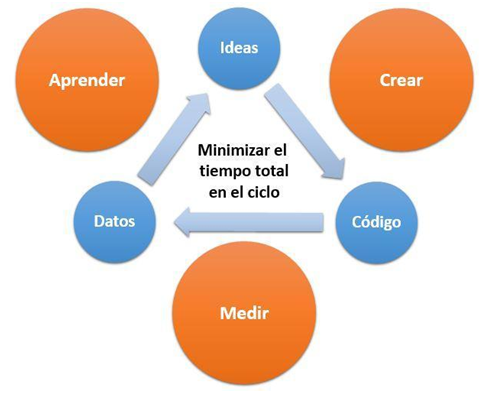
\includegraphics[scale=0.70]{../images/metodologia/agil.png}
    \caption{Metodología ágil}
    \label{fig:met_agil}
  \end{center}
\end{figure}


Por otra parte, es la manera que más natural resulta a la hora de desarrollar software pues se van completano hitos. Cada uno de ellos define una funcionalidad implementada por lo que si se desea abrir un nuevo camino \textit{(también llamados fork o roadmap)} en la aplicación tenemos varios puntos de partida evitando tener que empezar desde cero en caso de llegar a un \textit{punto muerto} en el desarrollo.

Las iteraciones se llevan acabo sobre las tareas de Implemetación, pruebas y documentación las cuales se detallan más abajo en éste capítulo.

http://mprende.co/gesti%C3%B3n/agile-scrum-y-lean-startups-metodolog%C3%ADas-de-desarrollo-%C3%A1gil-de-productos

\section{Análisis de requisitos}

A continuación se detallan los actores implicados en el sistema, requisitos funcionales y no funcionales, requisitos de almacenamiento, casos de uso y por último los diagramas generados para el desarrollo incluyendo en éste punto los bocetos ilustrativos de interfaz de la web.

\subsection{Actores}

Los actores que hacen uso del sistema son tres, \textbf{administrador}, el \textbf{aportador de información} y \textbf{usuario visitante}.

\bigskip
El \textbf{administrador} es el encargado de mantener el correcto funcionamiento de la aplicación y sus servicios.

\bigskip
El \textbf{aportador de información} puede ser cualquier usuario que decida configurar un dispositivo para añadir información, en éste caso creando un punto que recolecte datos y los remita al sistema.

\bigskip
El \textbf{usuario visitante} puede ser cualquier persona que consulte información en la aplicación, ya sea a través de la web o através de la plataforma para consultar todos los datos almacenados (en éste último caso el usuario debe tener un mínimo de conocimientos acerca de las consultas necesarias para obtener la información).

\subsection{Requisitos funcionales}

En ésta sección se describen las funcionalidades básicas que el sistema debe cubrir para dar el problema planteado como resuelto.

\begin{itemize}
  \item \textbf{RF-1.} Mapa web:
    \begin{itemize}
      \item \textbf{RF-1.1.} Desplegar la aplicación web.
      \item \textbf{RF-1.2.} Leer datos recibidos desde los clientes.
      \item \textbf{RF-1.2.} Mostrar los datos sin necesidad de refrescar la página.
    \end{itemize}
\end{itemize}

\begin{itemize}
  \item \textbf{RF-2.} Acceso libre a la información almacenada:
    \begin{itemize}
      \item \textbf{RF-2.1.} Proveer un sistema que sea capaz de mostrar los datos almacenados y filtrarlos según la conveniencia.
      \item \textbf{RF-2.2.} Proveer un sistema que sea capaz de extraer la información consultada.
    \end{itemize}
\end{itemize}

\begin{itemize}
  \item \textbf{RF-3.} Añadir información:
    \begin{itemize}
    \item \textbf{RF-3.1.} Un usuario podrá aportar información al sistema de manera independiente y autónoma.
  \end{itemize}
\end{itemize}

\begin{itemize}
  \item \textbf{RF-3.} Identificación de vehículos:
    \begin{itemize}
    \item \textbf{RF-3.1.} Filtrar la información entrante en forma de sonido e identificar si se trata de tráfico.
    \item \textbf{RF-3.2.} Hacer una distinción según el tipo de vehículo.
    \item \textbf{RF-3.3.} Si el dispositivo recolector se queda sin conexión, debe ser capaz de seguir almacenando los datos obtenidos y enviarlos cuando le sea posible.
    \end{itemize}
\end{itemize}


\subsection{Requisitos no funcionales}

Aquí se enumeran las propiedades ligadas al desarrollo e implementación que el sistema debe cumplir.

\begin{itemize}
  \item \textbf{RNF-0.} El software de terceros usado debe ser Open Source, así como los SO usados tanto para los servidores como para la Raspberry Pi.
  \item \textbf{RNF-1.} El módulo encargado de la detección del sonido estará desarrollado en {\tt Python} (por su simplicidad), las dependencias necesarias se detallarán en la sección de implementación. Además éste módulo debe aprovechar el procesamiento en paralelo para que su funcionamiento sea óptimo.
  \item \textbf{RNF-2.} La retransmisión de datos debe ser establecida en un intervalo de tiempo mínimo para garantizar que la aplicación actúa en tiempo real.
  \item \textbf{RNF-3.} El mapa web debe mostrar la información durante un breve periodo de tiempo para no acumular señales anteriores.
  \item \textbf{RNF-4.} Siempre que sea posible se automatizarán las interacciones con cualquier elemento del sistema mediante scripts.
  \item \textbf{RNF-5.} El código de la aplicación debe estar disponible en algún sistema de control de versiones y de manera pública.
\end{itemize}

\subsection{Requisitos de almacenamiento}

La información que se almacenará en el sistema se puede dividir en dos apartados, la información almacenada que sirve para representar los datos en la web y por otra parte la información que se almacena en una base de datos diseñada para consultas de datos masivas, que aunque tienen elementos similares difieren en algunos aspectos.

\begin{itemize}
  \item \textbf{RA-1.} Almacenamiento para la web.
  \begin{itemize}
    \item Timestamp de la señal recibida.
    \item Coordenadas de la señal recibida.
    \item Valor (numérico) de la señal recibida.
  \end{itemize}
  \item \textbf{RA-2.} Almacenamiento de datos masivo.
  \begin{itemize}
    \item Localización.
    \item Timestamp.
    \item Id del dispositivo.
    \item Valor de la señal.
  \end{itemize}
\end{itemize}

Obsérvese que no se almacena ningún dato personal luego a efectos prácticos, los artículos 7 y 8 de la LOPD en los que se detalla el tipo de datos de carácter sensible que hay que preservar con especial atención no tienen aplicación sobre RSMap.

http://www.boe.es/buscar/pdf/1999/BOE-A-1999-23750-consolidado.pdf#page=4&zoom=auto,-107,226

\newpage

\section{Casos de uso}

Debido a que RSMap es un servicio para proveer y aportar información, los casos de uso quedan simplificados de manera que la mayor parte de ellos hacen referencia a la aportación/consulta de datos.

\subsection{Descripción de actores}

\begin{itemize}
  \item \textbf{A-1.} Administrador.
  \begin{itemize}
   \item Descripción: Es el responsable del correcto funcionamiento de la aplicación.
   \item Tareas: Administración, mantenimiento y actualización de todos los elementos que conforman el sistema.
  \end{itemize}

  \item \textbf{A-2.} Usuario aportador de información.
  \begin{itemize}
   \item Descripción: Persona que se dispone a configurar un dispositivo para añadir información al sistema.
   \item Comentarios: Debe tener un conocimiento mínimo en sistemas operativos, concretamente en Linux (Raspberry Pi) para configurar el dispositivo y proceder a remitir información.
  \end{itemize}

  \item \textbf{A-2.} Usuario visitante.
  \begin{itemize}
   \item Descripción: Persona que se dispone a consultar los datos que almacena el sistema.
   \item Comentarios: Para la consulta de datos mediante la web no necesita ningún conocimiento, para la consulta en el almacenamiento masivo tal vez sea necesario tener conocimientos básicos en consultas. En cualquier caso se proveerán consultas predefinidas cuyos parámetros sean totalmente configurables.
  \end{itemize}
\end{itemize}

\subsection{Casos de uso}

\begin{itemize}
  \item \textbf{CU-1.} Desplegar servicio Web RSMap.
  \begin{itemize}
    \item Actores: Administrador.
    \item Tipo: Primario, esencial.
    \item Referencias:
    \item Precondición: Disponer de los ficheros de GitHub para lanzarla y una correcta configuración de puertos.
    \item Postcondición: Se ejecuta el servidor web de RSMap.
    \item Autor: \autor.
    \item Versión: 1.0.
    \item Propósito: Levantar una instancia de la web de RSMap.
    \item Resumen: El desarrollador puede actualizar la aplicación desde GitHub y lanzarla de manera fácil con nuevas funcionalidades.
  \end{itemize}
\end{itemize}
\begin{table}[!ht]
  \begin{center}
    \begin{tabular}{|l|l|l|l|}
      \hline
      \multicolumn{4}{|c|}{{\bf Caso de uso 1}}
      \\ \hline
      \multicolumn{2}{|c|}{{\bf Actor}} & \multicolumn{2}{c|}{{\bf Sistema}}
      \\ \hline
      {\it 1} &
      \begin{tabular}[c]{@{}l@{}}
        Administrador: descarga el\\
        repositorio de RSMap y\\
        lanza la aplicación web.
      \end{tabular} &
      &
      \\ \hline
      &
      &
      {\it 2} &
      \begin{tabular}[c]{@{}l@{}}
        El sistema sobre el que se  \\
        instala levanta un\\
        servicio web que contiene RSMap.\\
      \end{tabular}
      \\ \hline
    \end{tabular}
    \caption{Secuencia de CU-1}
    \label{table:cu_1}
  \end{center}
\end{table}

\begin{table}[!ht]
  \begin{center}
\begin{tabular}{|l|l|}
\hline
\multicolumn{2}{|c|}{{\bf Curso alterno}}
\\ \hline
{\it 2b} &
\begin{tabular}[c]{@{}l@{}}
  Si el servidor está funcionando, no se ejecuta \\
  la nueva instancia de la web.
\end{tabular}\\
\hline
\end{tabular}
\caption{Curso alterno de CU-1.}
\label{table:ca_cu_1}
  \end{center}
\end{table}

\newpage

\begin{itemize}
  \item \textbf{CU-2.} Configurar los clientes de RSMap.
  \begin{itemize}
    \item Actores: Administrador.
    \item Tipo: Primario, esencial.
    \item Referencias:
    \item Precondición: Disponer de los servidores necesarios para enviar la información.
    \item Postcondición: Los clientes remitirán los datos a donde el administrador desee.
    \item Autor: \autor.
    \item Versión: 1.0.
    \item Propósito: Permitir que un administrador defina nuevas localizaciones de almacenamiento.
    \item Resumen: El desarrollador puede actualizar la aplicación desde GitHub y ponerla a disposición de futuros usuarios aportadores de información.
  \end{itemize}
\end{itemize}
\begin{table}[!ht]
  \begin{center}
    \begin{tabular}{|l|l|l|l|}
      \hline
      \multicolumn{4}{|c|}{{\bf Caso de uso 2}}
      \\ \hline
      \multicolumn{2}{|c|}{{\bf Actor}} & \multicolumn{2}{c|}{{\bf Sistema}}
      \\ \hline
      {\it 1} &
      \begin{tabular}[c]{@{}l@{}}
        Administrador: descarga el\\
        repositorio de RSMapPi y\\
        lo configura con nuevos\\
        parámetros.
      \end{tabular} &
      &
      \\ \hline
      &
      &
      {\it 2} &
      \begin{tabular}[c]{@{}l@{}}
        La nueva configuración de\\
        los clientes permite enviar\\
        información a el destino\\
        seleccionado por el\\
        administrador\\.
      \end{tabular}
      \\ \hline
    \end{tabular}
    \caption{Secuencia de CU-2}
    \label{table:cu_1}
  \end{center}
\end{table}

\newpage

  \item \textbf{CU-3.} Consulta de datos mediante la web.
  \begin{itemize}
    \item Actores: Usuario visitante.
    \item Tipo: Primario, esencial.
    \item Referencias:
    \item Precondición: La aplicación web debe estar en funcionamiento.
    \item Postcondición: Se muestran identificadores en los lugares en los que se encuentra un dispositivo receptor y detecta tráfico.
    \item Autor: Cualquier usuario que acceda a la plataforma.
    \item Versión: 1.0.
    \item Propósito: Que el usuario tenga conocimiento de por que zonas existe tráfico.
    \item Resumen: El usuario entra en la web y puede ver el tráfico en tiempo real.
    \begin{table}[!ht]
      \begin{center}
	\begin{tabular}{|l|l|l|l|}
	  \hline
	  \multicolumn{4}{|c|}{{\bf Caso de uso 3}}
	  \\ \hline
	  \multicolumn{2}{|c|}{{\bf Actor}} & \multicolumn{2}{c|}{{\bf Sistema}}
	  \\ \hline
	  {\it 1} &
	  \begin{tabular}[c]{@{}l@{}}
	    Usuario: accede en la web\\
	    para visualizar el tráfico\\
	  \end{tabular} &
	  &
	  \\ \hline
	  &
	  &
	  {\it 2} &
	  \begin{tabular}[c]{@{}l@{}}
	    Muestra los marcas en los lugares \\
        en los que existe tráfico \\
        en ese momento. \\
	  \end{tabular}
	  \\ \hline
	\end{tabular}
	\caption{Secuencia de CU-3}
	\label{table:cu_2}
      \end{center}
    \end{table}

\begin{table}[!ht]
  \begin{center}
\begin{tabular}{|l|l|}
\hline
\multicolumn{2}{|c|}{{\bf Curso alterno}}
\\ \hline
{\it 2b} &
\begin{tabular}[c]{@{}l@{}}
  Si el no exiten dispositivos retransmitiendo\\
  la web informa al usuario.
\end{tabular}\\
\hline
\end{tabular}
\caption{Curso alterno de CU-3.}
\label{table:ca_cu_2}
  \end{center}
\end{table}

\newpage

  \item \textbf{CU-4.} Consulta de datos masivos.
  \begin{itemize}
    \item Actores: Usuario visitante.
    \item Tipo: Primario, esencial.
    \item Referencias:
    \item Precondición: La aplicación web debe estar en funcionamiento y la base de datos debe contener registros.
    \item Postcondición: Se muestran los datos según la consulta enviada.
    \item Autor: Cualquier usuario que acceda a la plataforma.
    \item Versión: 1.0.
    \item Propósito: Que el usuario tenga libre acceso a la información recopilada por los dispositivos que agregan información.
    \item Resumen: El usuario entra en la web y puede consultar los datos almacenados bajo las condiciones que el desee.
    \begin{table}[!ht]
      \begin{center}
    \begin{tabular}{|l|l|l|l|}
      \hline
      \multicolumn{4}{|c|}{{\bf Caso de uso 4}}
      \\ \hline
      \multicolumn{2}{|c|}{{\bf Actor}} & \multicolumn{2}{c|}{{\bf Sistema}}
      \\ \hline
      {\it 1} &
      \begin{tabular}[c]{@{}l@{}}
        Usuario: accede en la web\\
        y lanza una consulta \\
      \end{tabular} &
      &
      \\ \hline
      &
      &
      {\it 2} &
      \begin{tabular}[c]{@{}l@{}}
        Devuelve todas las entradas \\
        que cumplen las condiciones \\
        de la consulta. \\
      \end{tabular}
      \\ \hline
    \end{tabular}
    \caption{Secuencia de CU-4}
    \label{table:cu_3}
      \end{center}
    \end{table}
  \end{itemize}

  \begin{table}[!ht]
    \begin{center}
  \begin{tabular}{|l|l|}
  \hline
  \multicolumn{2}{|c|}{{\bf Curso alterno}}
  \\ \hline
  {\it 2b} &
  \begin{tabular}[c]{@{}l@{}}
    Si no existen datos en base a la consulta \\
    el sistema no devuelve nada y se muestra un error.
  \end{tabular}\\
  \hline
  \end{tabular}
  \caption{Curso alterno de CU-4.}
  \label{table:ca_cu_1}
    \end{center}
  \end{table}

\newpage

  \item \textbf{CU-5.} Añadir nuevos dispositivos.
  \begin{itemize}
    \item Actores: Aportador de información.
    \item Tipo: Primario, esencial.
    \item Referencias:
    \item Precondición: Tiene un dispositivo capaz de remitir información al sistema.
    \item Postcondición: Los datos que remitidos quedan guardados en el sistema.
    \item Autor: Administrador, Usuario Aportador.
    \item Versión: 1.0.
    \item Propósito: Que cualquier usuario pueda aportar información al sistema.
    \item Resumen: El usuario se descarga desde GitHub el cliente y lo ejecuta para enviar información del tráfico en su localización.
    \begin{table}[!ht]
      \begin{center}
	\begin{tabular}{|l|l|l|l|}
	  \hline
	  \multicolumn{4}{|c|}{{\bf Caso de uso 5}}
	  \\ \hline
	  \multicolumn{2}{|c|}{{\bf Actor}} & \multicolumn{2}{c|}{{\bf Sistema}}
	  \\ \hline
	  {\it 1} &
	  \begin{tabular}[c]{@{}l@{}}
	    Usuario: se descarga el cliente\\
	    y lo configura para el envío\\
	  \end{tabular} &
	  &
	  \\ \hline
	  &
	  &
	  {\it 2} &
	  \begin{tabular}[c]{@{}l@{}}
	    Almacena los datos remitidos \\
        por el usuario aportador. \\
	  \end{tabular}
	  \\ \hline
	\end{tabular}
	\caption{Secuencia de CU-5}
	\label{table:cu_4}
      \end{center}
    \end{table}
  \end{itemize}

\end{itemize}

\newpage
\section{Diagramas}
\subsection{Diagrama de paquetes}

En este diagrama podemos observar las dependencias que existen entre los distintos paquetes del sistema y como el paquete \textbf{IOT} es el elemento central sobre el que se apoyan los demás. El paquete \textbf{Raspberry Pi} es dependiente del paquete de \textbf{IOT} debido a que \textbf{IOT} es el encargado de definir como los clientes van a escribir en el almacenamiento masivo. A su vez el paquete \textbf{RSMap web} es dependiente de \textbf{Raspberry Pi} debio a que las señales de vehículos se mandarán directamente a la plataforma web gracias a la \textbf{API Rest}.

Por otra parte tenemos el paquete \textbf{Visualizador} el cual usa al paquete \textbf{Almacenamiento masivo} para proveerse de información que mostrar. Por último \textbf{Almacenamiento masivo} es dependiente de \textbf{IOT} debido a que los esquemas (estructura de almacenamiento) se definen en \textbf{IOT} y éste se encarga de definirlas en el \textbf{Almacenamiento masivo}.

\begin{figure}[!ht]
  \begin{center}
    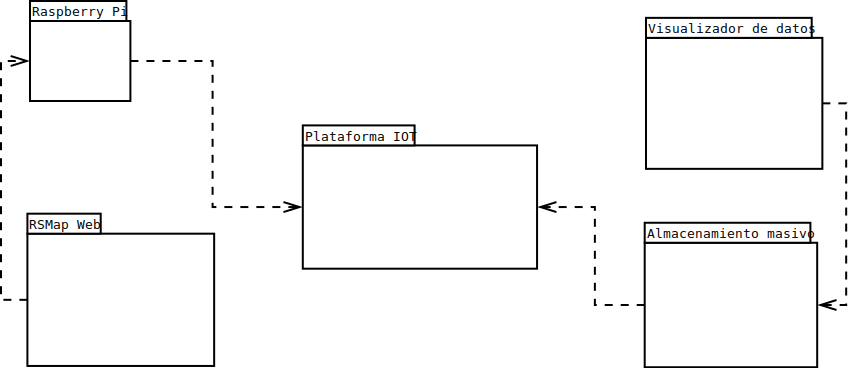
\includegraphics[scale=0.50]{../images/diag_plan/paquetes.png}
    \caption{Diagrama de paquetes}
    \label{fig:paquetes}
  \end{center}
\end{figure}

\newpage

\subsection{Diagrama arquitectónico}

En ésta sección se detallan los elementos de la estructura que compondrá la aplicación. Debido a que los dispositivos receptores \textbf{(Raspberry pi)} poseen una estructura interna la cual merece atención se han detallado por separado el diagrama de los receptores \textit{(figura 4.5)} y el del sistema completo \textit{(figura 4.6)}.

\bigskip

El sistema recibirá la entrada de audio mediante un micrófono, tras ésto el módulo encargao de recolectar los datos efectuará un filtrado previo evitando así analizar datos innecesarios de ésta manera minimizamos la sobrecarga del dispositivo. Tras ésto se procede a analizar los datos que han pasado el primer filtro. Por último se envían los datos con los resultados a los distintos sistemas de almacenamiento que se detallan en el siguiente diagrama.

\bigskip

\begin{figure}[!ht]
  \begin{center}
  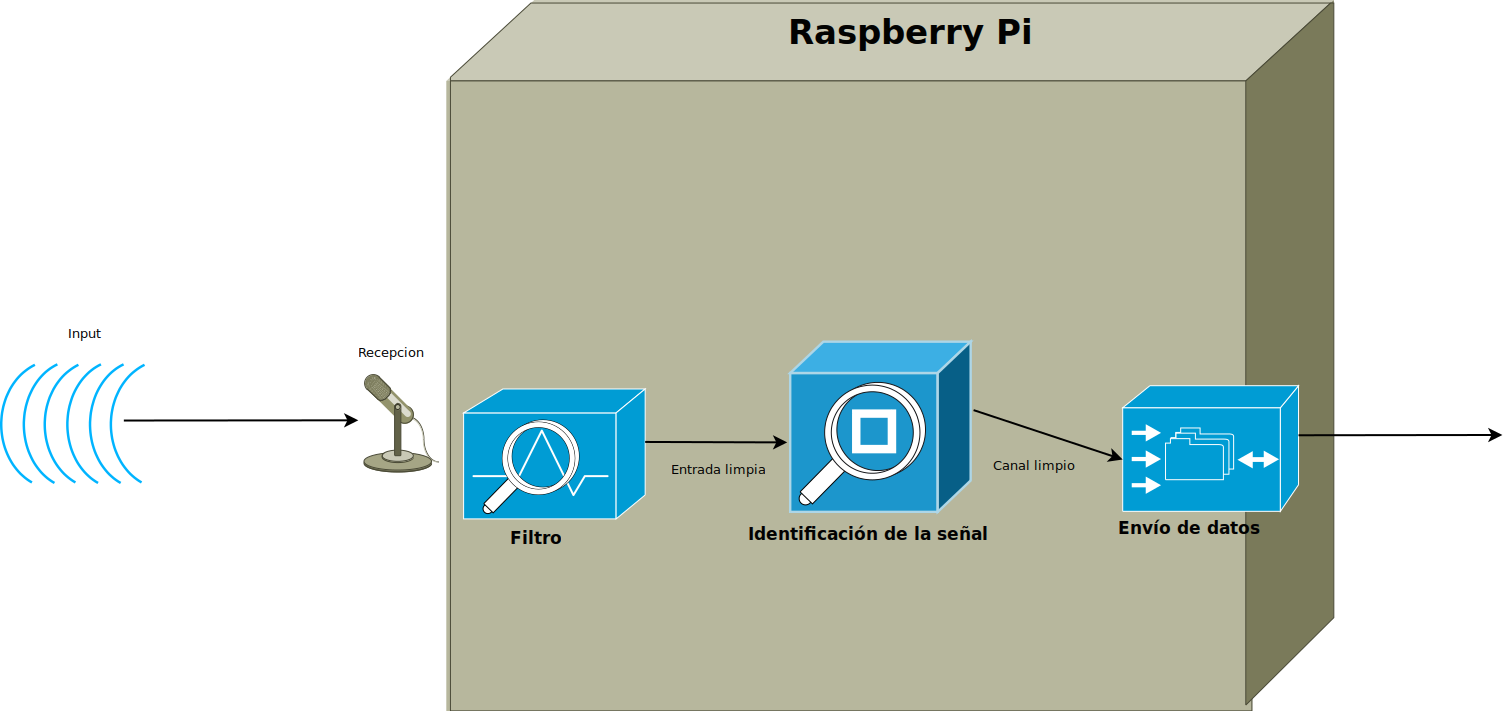
\includegraphics[scale=0.25]{../images/diag_plan/diag_arqu_pi.png}
  \caption{Arquitectura Raspberry Pi}
  \label{fig:ar_rpi}
  \end{center}
\end{figure}

Ahora se muestra cual será la estructura en conjunto de todos los elementos que conforman \textbf{RSMap.}


Tras haber analizado el comportamiento de los dispositivos receptores, el siguiente elemento a destacar es la plataforma IOT, la manera de transmitir la información según la configuración establecida, en la que se detalla a donde tienen que remitir los dispositivos la información así como los propios modelos de datos. Los receptores harán uso de ésto para enviar la información a \textbf{Almacenamiento masivo}.

Por otra parte, también realizarán envíos a el servidor web indicando cuando pasa un vehículo por la localización en la que se encuentren, el cual atenderá las peticiones de los clientes que soliciten acceder a RSMap.

Como último elemento nos queda \textbf{Visualizador}, que actúa a modo de Notebook y es el encargado de realizar las consultas que el usuario defina a \textbf{Almacenamiento masivo} para poder acceder a los datos que han almacenado los dispositivos receptores.

\begin{figure}[!ht]
  \begin{center}
  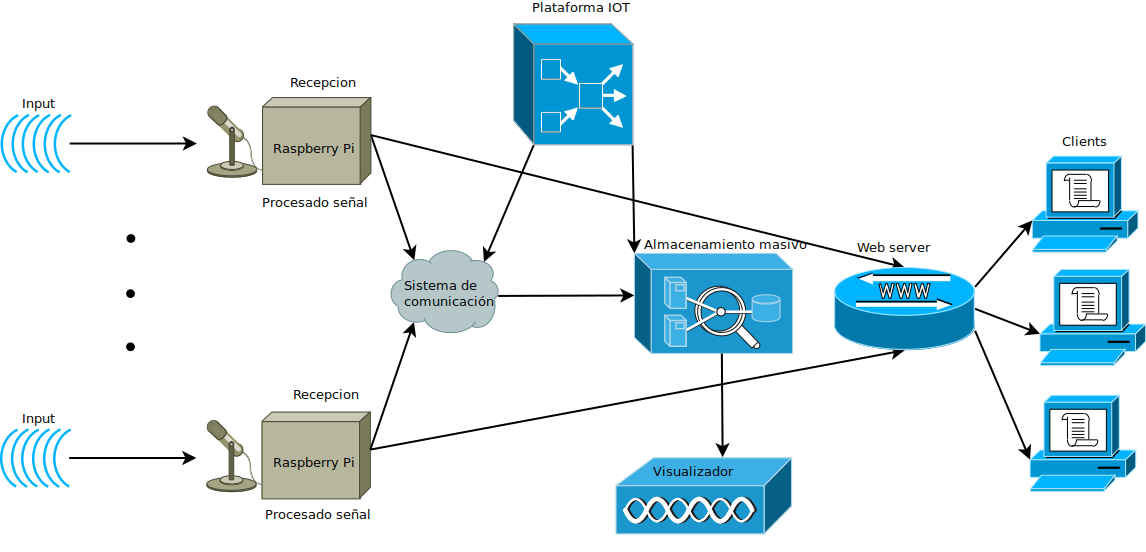
\includegraphics[scale=0.35]{../images/diag_plan/diag_arqu.png}
  \caption{Arquitectura de RSMap}
  \label{fig:ar_rsmap}
  \end{center}
\end{figure}

\newpage

\subsection{Diagrama de clases}

\begin{figure}[!ht]
  \begin{center}
  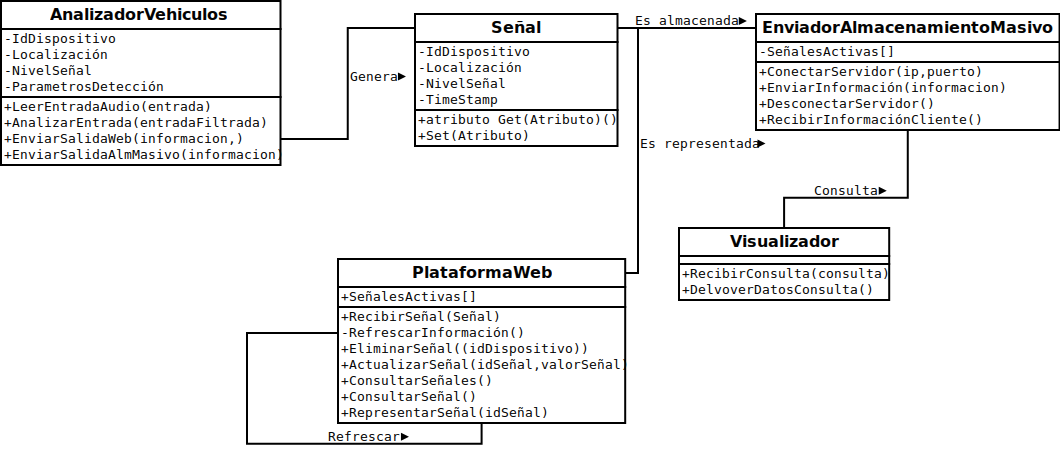
\includegraphics[scale=0.60, angle=90]{../images/diag_plan/clases.png}
  \caption{Diagrama de clases}
  \label{fig:ar_rsmap}
  \end{center}
\end{figure}

\newpage

\subsection{Diagramas de casos de uso}

Ahora detallaremos de qué manera pueden interactuar los distintos actores con el sistema. A modo de vista general se proporciona un diagrama de Caso de uso global.

\begin{figure}[!ht]
  \begin{center}
    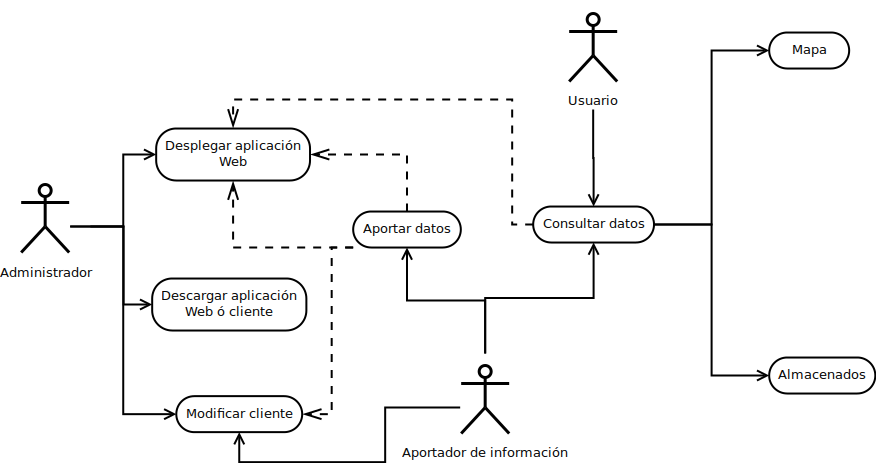
\includegraphics[scale=0.45]{../images/diag_plan/cu_gen.png}
    \caption{Caso de uso general}
    \label{fig:cu_admin}
  \end{center}
\end{figure}



El administrador tiene capacidad para realizar actividades de mantenimiento y chequeo de los parámetros usados, así como generar nuevas configuraciones.
\begin{figure}[!ht]
  \begin{center}
    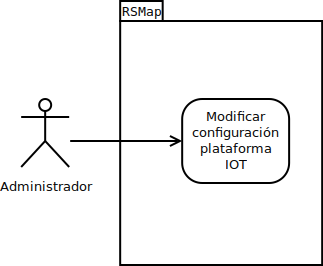
\includegraphics[scale=0.45]{../images/diag_plan/cu_admin.png}
    \caption{Caso de uso del administrador}
    \label{fig:cu_admin}
  \end{center}
\end{figure}

\newpage

En segundo lugar tenemos el usuario que puede consultar los datos bien sea mediante el mapa web, el cual sólo indica señales en los puntos en los que pasen vehículos, mientras que mediante el visualizador de datos masivos podrá consultar el conjunto total de información almacenada.

\begin{figure}[!ht]
  \begin{center}
  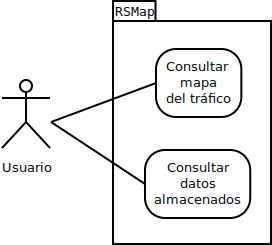
\includegraphics[width=0.45\textwidth]{../images/diag_plan/cu_usuario.png}
  \caption{Caso de uso del usuario}
  \label{fig:cu_usuario}
  \end{center}
\end{figure}

Por último el usuario aportador podrá bajarse el código fuente desde GitHub y podrá ejecutarlo para enviar la información a RSMap. Como se trata de una especialización del Usuario, se da por entendido que también tendrá acceso a los datos.

\begin{figure}[!ht]
  \begin{center}
  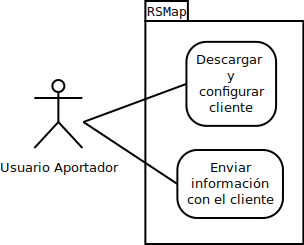
\includegraphics[width=0.45\textwidth]{../images/diag_plan/cu_usuario_aportador.png}
  \caption{Caso de uso del usuario aportador}
  \label{fig:cu_uaportador}
  \end{center}
\end{figure}

\newpage


\subsection{Diagramas de secuencia}

Ahora se detallan los pasos de forma generalizada que cada tipo de usuario realiza y qué efectos desencadenan sobre el sistema.

\begin{figure}[!h]
  \begin{center}
  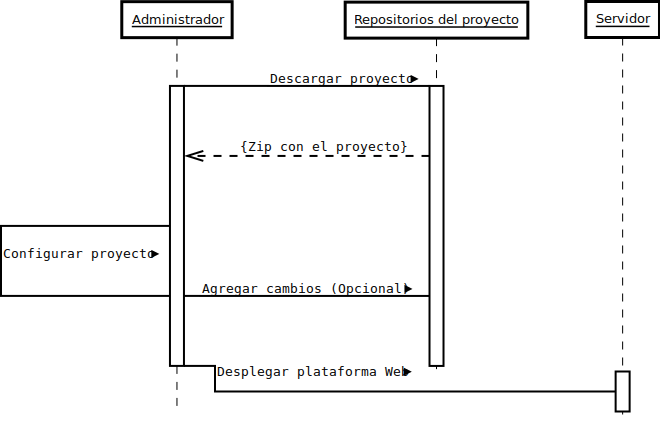
\includegraphics[scale=0.45]{../images/diag_plan/seq_admin.png}
  \caption{Diagrama de secuencia del Administrador}
  \label{fig:ar_rsmap}
  \end{center}
\end{figure}

\newpage

\begin{figure}[!h]
  \begin{center}
  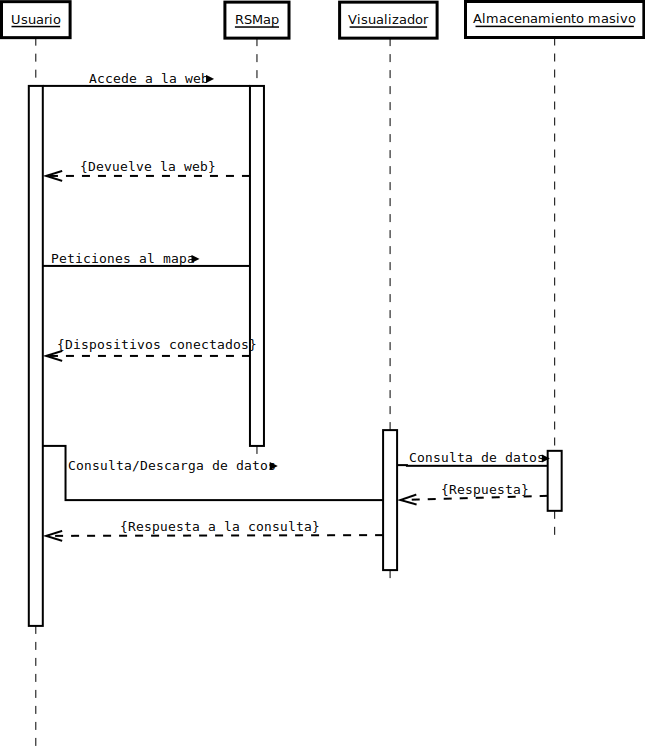
\includegraphics[scale=0.5]{../images/diag_plan/seq_user.png}
  \caption{Diagrama de secuencia del Usuario}
  \label{fig:ar_rsmap}
  \end{center}
\end{figure}

\newpage

\begin{figure}[!h]
  \begin{center}
  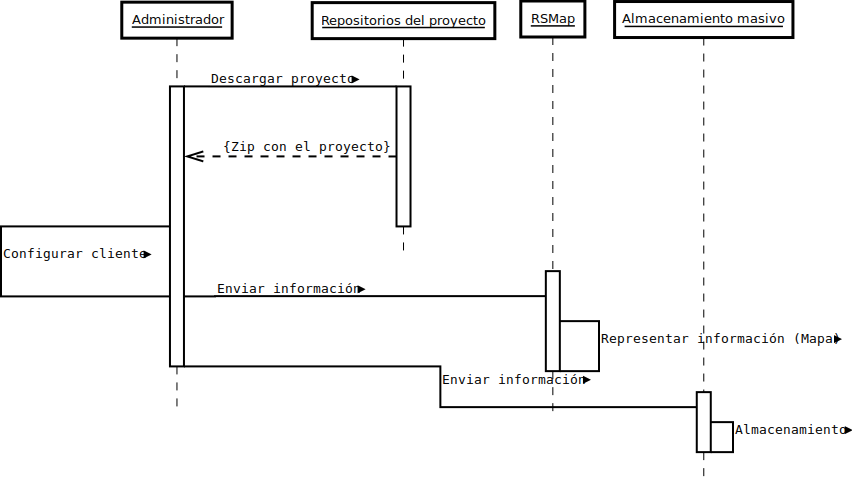
\includegraphics[scale=0.45]{../images/diag_plan/seq_user_ap.png}
  \caption{Diagrama de secuencia del Usuario Aportador}
  \label{fig:ar_rsmap}
  \end{center}
\end{figure}

\newpage

\subsection{Diagramas de interfaz}

Aquí se presentan dos pequeños esbozos de una aproximación a la interfaz de la web, no se ha entrado en mucho nivel de detalle debido a que la idea es usar una plantilla de Bootstrap y adaptarla a las necesidades, en cualquier caso el aspecto deberá asemejarse al ilustrado en la \textit{figura 4.7} para la página principal y para la página del mapa el de la \textit{figura 4.8}.

\begin{figure}[!ht]
  \begin{center}
  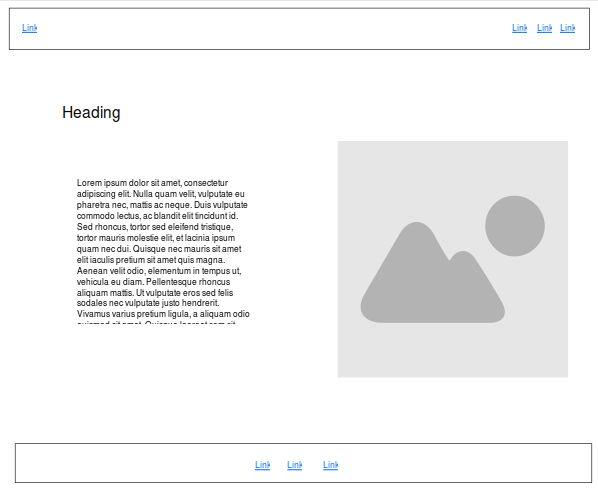
\includegraphics[scale=0.6]{../images/diag_plan/ui_general.png}
  \caption{Boceto de la página principal}
  \label{fig:ar_rsmap}
  \end{center}
\end{figure}

\newpage

\begin{figure}[!ht]
  \begin{center}
  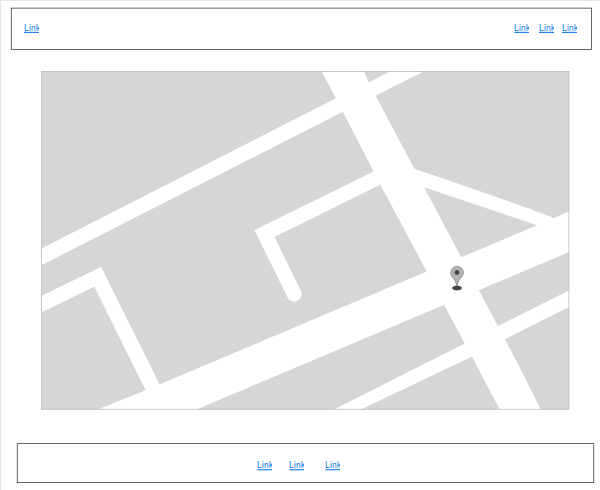
\includegraphics[scale=0.65]{../images/diag_plan/ui_mapa.png}
  \caption{Boceto de la página del mapa}
  \label{fig:ar_rsmap}
  \end{center}
\end{figure}
